\documentclass{beamer}
%
% Common preamble for all three parts.
%

\usepackage[english]{babel}
\usepackage{amsmath}
\usepackage{color}
\usepackage{minted}
\usepackage{hyperref}
\usepackage{multicol}
\usepackage{tabularx}
\usepackage{tikz}

% only inline todonotes work
\usepackage{xkeyval}
\usepackage[textsize=small]{todonotes}
\presetkeys{todonotes}{inline}{}

\usetikzlibrary{shapes,arrows,positioning,shadows}

% no nav buttons
\usenavigationsymbolstemplate{}

\newcommand{\bftt}[1]{\textbf{\texttt{#1}}}
\newcommand{\comment}[1]{{\color[HTML]{008080}\textit{\textbf{\texttt{#1}}}}}
\newcommand{\cmd}[1]{{\color[HTML]{008000}\bftt{#1}}}
\newcommand{\bs}{\char`\\}
\newcommand{\cmdbs}[1]{\cmd{\bs#1}}
\newcommand{\lcb}{\char '173}
\newcommand{\rcb}{\char '175}
\newcommand{\cmdbegin}[1]{\cmdbs{begin\lcb}\bftt{#1}\cmd{\rcb}}
\newcommand{\cmdend}[1]{\cmdbs{end\lcb}\bftt{#1}\cmd{\rcb}}

\newcommand{\wllogo}{\textbf{Overleaf}}

% this is where the example source files are loaded from
% do not include a trailing slash
\newcommand{\fileuri}{https://raw.githubusercontent.com/GiancarloSucci/IDSEPC/main/LaTeX}

\newcommand{\wlserver}{https://www.overleaf.com}
\newcommand{\wlnewdoc}[1]{\wlserver/docs?snip\_uri=\fileuri/#1\&splash=none}

\def\tikzname{Ti\emph{k}Z}

% from http://tex.stackexchange.com/questions/5226/keyboard-font-for-latex
\newcommand*\keystroke[1]{%
  \tikz[baseline=(key.base)]
    \node[%
      draw,
      fill=white,
      drop shadow={shadow xshift=0.25ex,shadow yshift=-0.25ex,fill=black,opacity=0.75},
      rectangle,
      rounded corners=2pt,
      inner sep=1pt,
      line width=0.5pt,
      font=\scriptsize\sffamily
    ](key) {#1\strut}
  ;
}
\newcommand{\keystrokebftt}[1]{\keystroke{\bftt{#1}}}

% stolen from minted.dtx
\newenvironment{exampletwoup}
  {\VerbatimEnvironment
   \begin{VerbatimOut}{example.out}}
  {\end{VerbatimOut}
   \setlength{\parindent}{0pt}
   \fbox{\begin{tabular}{l|l}
   \begin{minipage}{0.55\linewidth}
     \inputminted[fontsize=\small,resetmargins]{latex}{example.out}
   \end{minipage} &
   \begin{minipage}{0.35\linewidth}
     \input{example.out}
   \end{minipage}
   \end{tabular}}}

\newenvironment{exampletwouptiny}
  {\VerbatimEnvironment
   \begin{VerbatimOut}{example.out}}
  {\end{VerbatimOut}
   \setlength{\parindent}{0pt}
   \fbox{\begin{tabular}{l|l}
   \begin{minipage}{0.55\linewidth}
     \inputminted[fontsize=\scriptsize,resetmargins]{latex}{example.out}
   \end{minipage} &
   \begin{minipage}{0.35\linewidth}
     \setlength{\parskip}{6pt plus 1pt minus 1pt}%
     \raggedright\scriptsize\input{example.out}
   \end{minipage}
   \end{tabular}}}

\newenvironment{exampletwouptinynoframe}
  {\VerbatimEnvironment
   \begin{VerbatimOut}{example.out}}
  {\end{VerbatimOut}
   \setlength{\parindent}{0pt}
   \begin{tabular}{l|l}
   \begin{minipage}{0.55\linewidth}
     \inputminted[fontsize=\scriptsize,resetmargins]{latex}{example.out}
   \end{minipage} &
   \begin{minipage}{0.35\linewidth}
     \setlength{\parskip}{6pt plus 1pt minus 1pt}%
     \raggedright\scriptsize\input{example.out}
   \end{minipage}
   \end{tabular}}

%\title{An Interactive Introduction to \LaTeX}
%\author{Dr John D. Lees-Miller}
%\titlegraphic{%
%
\includegraphics[height=36pt]{overleaf}\\[1em]
%\includegraphics[height=24pt]{UoB-logo}
%}


%
% Choose how your presentation looks.
% For more themes, color themes and font themes, see:
% http://deic.uab.es/~iblanes/beamer_gallery/index_by_theme.html
%
\mode<presentation>
{
  \usetheme{Madrid}      % or try Darmstadt, Madrid, Warsaw, ...
  \usecolortheme{seahorse} % or try albatross, beaver, crane, ...
  \usefonttheme{serif}  % or try serif, structurebold, ...
  \setbeamertemplate{navigation symbols}{}
  \setbeamertemplate{caption}[numbered]
  \usepackage{amsmath}
  \usepackage{tcolorbox}
  \usepackage[export]{adjustbox}
  \tcbuselibrary{most}
  \usepackage{arydshln}
  \usepackage{eurosym}
 %\usepackage{enumitem}
%\usepackage{enumerate}
  %\usepackage[shortlabels]{enumitem}
} 


\definecolor{myblue}{RGB}{65,105,225} 
\definecolor{myorange}{RGB}{250,190,0}

\setbeamercolor{structure}{fg=white,bg=myorange}
\setbeamercolor*{palette primary}{fg=myblue,bg=myorange}
\setbeamercolor*{palette secondary}{fg=white,bg=myblue}
\setbeamercolor*{palette tertiary}{bg=myblue,fg=white}
\setbeamercolor*{palette quaternary}{fg=white,bg=myorange!50}

\setbeamercolor{frametitle}{fg=black!90!myblue}

\setbeamercolor{section in head/foot}{fg=white,bg=myblue}
\setbeamercolor{author in head/foot}{fg=black,bg=myorange}
\setbeamercolor{title in head/foot}{fg=white,bg=myblue}

\setbeamertemplate{navigation symbols}{}

\defbeamertemplate*{headline}{mytheme}
{%
  \begin{beamercolorbox}[ht=2.25ex,dp=3.75ex]{section in head/foot}
    \insertnavigation{\paperwidth}
  \end{beamercolorbox}%
}%

\defbeamertemplate*{footline}{mytheme}
{
  \leavevmode%
  \hbox{%
  \begin{beamercolorbox}[wd=.5\paperwidth,ht=2.25ex,dp=1ex,right]{author in head/foot}%
    \usebeamerfont{author in head/foot}\insertshortauthor\hspace*{2em}
  \end{beamercolorbox}%
  \begin{beamercolorbox}[wd=.5\paperwidth,ht=2.25ex,dp=1ex,left]{title in head/foot}%
    \usebeamerfont{title in head/foot}\hspace*{2em}\insertshortsubtitle\hspace*{2em}
    \insertframenumber{} / \inserttotalframenumber
  \end{beamercolorbox}}%
  \vskip0pt%
}



\usepackage[english]{babel}
\usepackage[utf8x]{inputenc}
\usepackage{xcolor}
\usepackage{listings}
\usepackage{pgf}  
\usepackage{textpos}
\usepackage{tabulary}
\usepackage{scrextend}
\usepackage{hyperref}
\usepackage{setspace}
\usepackage{rotating}
\lstset
{
    language=[LaTeX]TeX,
    breaklines=true,
    basicstyle=\tt\scriptsize,
    %commentstyle=\color{green}
    keywordstyle=\color{blue},
    %stringstyle=\color{black}
    identifierstyle=\color{magenta},
}

\usepackage{stackengine}
\def\Ruble{\stackengine{.67ex}{%
  \stackengine{.48ex}{\textsf{P}}{\rule{.8ex}{.12ex}\kern.6ex}{O}{r}{F}{F}{L}%
  }{\rule{.8ex}{.12ex}\kern.6ex}{O}{r}{F}{F}{L}\kern-.1ex}



%----------------------------------------------------------------------------------------
%	TITLE PAGE
%----------------------------------------------------------------------------------------
%\logo{\pgfbox[top]{
\includegraphics[width=1.6cm]{logo-iu.png}}}
\title[L01]{Intr. alla data science e al pensiero computazionale \\ Lezione 2 e 3: Scrivere documenti con un linguaggio di programmazione -- \LaTeX{}} % The short title appears at the bottom of every slide, the full title is only on the title page

\author[{\tiny Giancarlo Succi}]{Giancarlo Succi \\ sulla base del lavoro originale John D. Lees-Miller \\ I dettagli nel seguito} % Your name
\institute[unibo] % Your institution as it will appear on the bottom of every slide, may be shorthand to save space

\date{} % Date, can be changed to a custom date
%\pgfdeclareimage[width=2.5cm]{logo}{logo-iu.png}
%\logo{\pgfuseimage{logo}{\vspace{10pt}}}

\setbeamertemplate{navigation symbols}{}
\AtBeginSection[]
{
        \begin{frame}<beamer>{Outline}
                \tableofcontents[currentsection]
        \end{frame}
}
\begin{document}
\begin{frame}
\titlepage % Print the title page as the first slide
\end{frame}

%=============================================

\addtobeamertemplate{frametitle}{}{%
\begin{textblock*}{10mm}(-0.01mm,-0.95cm)

\includegraphics[width=0.9cm]{unibo-logo.png}
\end{textblock*}}

%=============================================
\begin{frame}[label={L:Fonti}]
{\centerline{Fonti}}
\begin{itemize}
    \item Tutte queste diapositive provengono dal lavoro di John Lees-Miller presente sul sito \url{https://github.com/jdleesmiller/latex-course} e sono state tradotte e adattate dal docente del corso, essendo state messe a disposizione dall'autore con una licenza idonea. 
    \item Ulteriori fonti verranno dettagliate in seguito.
\end{itemize}
\end{frame}

\begin{frame}
{\centerline{\LaTeX{} $\ldots{}$ Perch\'{e}?}}
\begin{itemize}
\item Rende i documenti bellissimi!
\begin{itemize}
\item Anche quelli con formule e dati -- ideale per i professionisti dei dati e della transizione digitale
\end{itemize}
%
\item \`{E} stato creato da scienziati per scienziati.
\begin{itemize}
\item Ed \`{e} mantenuto da una comunit\`{a} vasta in tutto il mondo.
\end{itemize}
%
\item \`{E} molto potente e pu\`{o} anche essere esteso.
\begin{itemize}
\item Ci sono estensioni particolari per articoli, presentazioni, fogli elettronici, libri e ogni altra possibile necessit\`{a}
\end{itemize}
\end{itemize}
\end{frame}

%%%%%%%%%%%%%%%%%%%%%%%%%%%%%%%%%%%%%%%%%%%%%%%%%%%%%%%%%%%%%%%%%%%%%%%%%%%%%%%
%%%%%%%%%%%%%%%%%%%%%%%%%%%%%%%%%%%%%%%%%%%%%%%%%%%%%%%%%%%%%%%%%%%%%%%%%%%%%%%
%%%%%%%%%%%%%%%%%%%%%%%%%%%%%%%%%%%%%%%%%%%%%%%%%%%%%%%%%%%%%%%%%%%%%%%%%%%%%%%

\begin{frame}[fragile]{\centerline{L'idea di fondo}}
\begin{itemize}
\item Si scrivono i documenti focalizzandosi sul \texttt{testo}, sul suo significato senza preoccuparsi della formattazione
\item Si aggiungono \cmd{comandi} che descrivono la veste grafica e la struttura dei documenti
\item Il programma \texttt{latex} analizza il \texttt{testo} ed i   \cmd{comandi} e produce un documento cotto a puntino. 
\end{itemize}
\vskip 2ex
\begin{center}
\begin{minted}[frame=single]{latex}
La nebbia in Italia si trova \emph{soprattutto} a Milano.
\end{minted}
\vskip 2ex
\tikz\node[single arrow,fill=gray,font=\ttfamily\bfseries,%
  rotate=270,xshift=-1em]{latex};
\vskip 2ex
\fbox{La nebbia in Italia si trova \emph{soprattutto} a Milano.}
\end{center}
\end{frame}

%%%%%%%%%%%%%%%%%%%%%%%%%%%%%%%%%%%%%%%%%%%%%%%%%%%%%%%%%%%%%%%%%%%%%%%%%%%%%%%
\begin{frame}[fragile]{\centerline{Esempi di comandi}}
\begin{exampletwoup}
\begin{itemize}
\item Espresso
\item Cappuccino
\item Caff\`{e} latte
\end{itemize}
\end{exampletwoup}
\vskip 2ex
\begin{exampletwoup}
\begin{figure}

\includegraphics{A2022.IDSEPCLaTeX/gerbil.jpg}
\end{figure}
\end{exampletwoup}
\vskip 2ex
\begin{exampletwoup}
\begin{equation}
\alpha + \beta + 1
\end{equation}
\end{exampletwoup}

\tiny{Licenza per le immagini: \href{https://pixabay.com/en/animal-apple-attractive-beautiful-1239390/}{CC0}}
\end{frame}

%%%%%%%%%%%%%%%%%%%%%%%%%%%%%%%%%%%%%%%%%%%%%%%%%%%%%%%%%%%%%%%%%%%%%%%%%%%%%%%
%%%%%%%%%%%%%%%%%%%%%%%%%%%%%%%%%%%%%%%%%%%%%%%%%%%%%%%%%%%%%%%%%%%%%%%%%%%%%%%
%%%%%%%%%%%%%%%%%%%%%%%%%%%%%%%%%%%%%%%%%%%%%%%%%%%%%%%%%%%%%%%%%%%%%%%%%%%%%%%
\begin{frame}[fragile]{\centerline{L'approccio da seguire}}

\begin{itemize}
\item Bisogna innanzitutto focalizzarsi sul contenuto, ricordandosi Catone ``Rem tene, verba sequentur'' ... ``Rem tene, species sequetur''
\item I comandi vanno poi usati per specificare di che cosa si tratta e non come deve apparire.
\item Quindi si lascia \LaTeX{} a fare il suo lavoro.
\item La presentazione grafica pu\`{o} poi essere adattara configurando appropriatamente i comandi.
\end{itemize}
\end{frame}

%%%%%%%%%%%%%%%%%%%%%%%%%%%%%%%%%%%%%%%%%%%%%%%%%%%%%%%%%%%%%%%%%%%%%%%%%%%%%%%
%%%%%%%%%%%%%%%%%%%%%%%%%%%%%%%%%%%%%%%%%%%%%%%%%%%%%%%%%%%%%%%%%%%%%%%%%%%%%%%
%%%%%%%%%%%%%%%%%%%%%%%%%%%%%%%%%%%%%%%%%%%%%%%%%%%%%%%%%%%%%%%%%%%%%%%%%%%%%%%
%\section{The Basics}

%%%%%%%%%%%%%%%%%%%%%%%%%%%%%%%%%%%%%%%%%%%%%%%%%%%%%%%%%%%%%%%%%%%%%%%%%%%%%%%
%%%%%%%%%%%%%%%%%%%%%%%%%%%%%%%%%%%%%%%%%%%%%%%%%%%%%%%%%%%%%%%%%%%%%%%%%%%%%%%
%%%%%%%%%%%%%%%%%%%%%%%%%%%%%%%%%%%%%%%%%%%%%%%%%%%%%%%%%%%%%%%%%%%%%%%%%%%%%%%
\begin{frame}[fragile]{\centerline{Fiato alle trombe!}}
\begin{itemize}
\item Un documento \LaTeX{} minimo:
\inputminted[frame=single]{latex}{A2022.IDSEPCLaTeX/minimale.tex}
\item I comandi iniziano con un \emph{backslash} \keystrokebftt{\bs}.
\item Ogni documento inizia col comando \cmdbs{documentclass} che specifica la natura del documento stesso.
\item L'\emph{argomento} in parentesi graffe \keystrokebftt{\{} \keystrokebftt{\}} comunica a \LaTeX{} il tipo di documento che stiamo creando -- nel nostro caso un articolo, in inglese \bftt{article}.
\item Il simbolo di percentuale \keystrokebftt{\%} inizia una regione di testo che viene usata per fornire un commento per i lettori del testo \LaTeX{} e non del documento finale, in inglese si chiama \emph{comment} 
\begin{itemize}
\item \LaTeX{} ignora tutto il testo fino alla fine della linea.
\end{itemize}
\end{itemize}
\end{frame}

%%%%%%%%%%%%%%%%%%%%%%%%%%%%%%%%%%%%%%%%%%%%%%%%%%%%%%%%%%%%%%%%%%%%%%%%%%%%%%%
%%%%%%%%%%%%%%%%%%%%%%%%%%%%%%%%%%%%%%%%%%%%%%%%%%%%%%%%%%%%%%%%%%%%%%%%%%%%%%%
%%%%%%%%%%%%%%%%%%%%%%%%%%%%%%%%%%%%%%%%%%%%%%%%%%%%%%%%%%%%%%%%%%%%%%%%%%%%%%%
\begin{frame}[fragile]{\centerline{Usando \wllogo}}
\begin{itemize}
\item Overleaf \`{e} un sito web \textit{parzialmente} gratuito per scrivere documenti in \LaTeX.
\item Processa automaticamente il documento \LaTeX{} e visualizza il risultato.
\item In questo modo non occorre installare \LaTeX{} sul proprio calcolatore
\item Questo \`{e} il motivo del suo uso in questo corso
\item Gli svantaggi:
\begin{itemize}
\item occorre praticamente essere online nella versione gratuita
\item la versione gratuita ha limitazioni di dimensioni, collaboratori, ecc;
\end{itemize}
\end{itemize}

\end{frame}

\begin{frame}[fragile]{\centerline{Proviamo \wllogo}}
\begin{itemize}
\begin{center}
\fbox{\href{\wlnewdoc{minimale.tex}}{%
Cliccare qui per aprire un documento di esempio in \wllogo{}}}
\\[1ex]\scriptsize{}
\`{E} preferibile usare come browser  \href{http://www.google.com/chrome}{Google Chrome},  \href{http://www.mozilla.org/en-US/firefox/new/}{FireFox}, o \href{https://www.apple.com/safari/}{Safari}.
\end{center}
\vskip 2ex
\item A casa provate su \wllogo ~ gli esempi che stiamo analizzando in classe.
\item \textbf{La pratica \`{e} una parte essenziale per la comprensione dell'importanza di questo strumento di produzione di documenti!}
\end{itemize}
\end{frame}

%%%%%%%%%%%%%%%%%%%%%%%%%%%%%%%%%%%%%%%%%%%%%%%%%%%%%%%%%%%%%%%%%%%%%%%%%%%%%%%
%%%%%%%%%%%%%%%%%%%%%%%%%%%%%%%%%%%%%%%%%%%%%%%%%%%%%%%%%%%%%%%%%%%%%%%%%%%%%%%
%%%%%%%%%%%%%%%%%%%%%%%%%%%%%%%%%%%%%%%%%%%%%%%%%%%%%%%%%%%%%%%%%%%%%%%%%%%%%%%
\begin{frame}[fragile]{\centerline{Proviamo ad elaborare un testo}}
\small
\begin{itemize}
\item Scrivete il vostro testo tra \cmdbegin{document} e \cmdend{document}.
\item Nella maggior parte dei casi potete scrivere liberamente senza preoccuparvi in alcun modo della formattazione.
\begin{exampletwouptiny}
Le parole sono separate     da uno
o pi\`{u} spazi.

I paragrafi sono separati da una
o pi\`{u} linee bianche.

\end{exampletwouptiny}
\item Gli spazi e gli a capo singoli nel testo originario (detto anche \textit{testo sorgente}) sono di fatto ignorati e il testo \`{e} reso in quella che \`{e} ritenuta la forma ideale a prescindere da essi.
\begin{exampletwouptiny}
La nebbia      in Italia si trova
      soprattutto    a
Milano.
\end{exampletwouptiny}
\end{itemize}
\end{frame}

\begin{frame}[fragile]{\centerline{Le lettere accentate}}
\small
\begin{itemize}
\item Per le lettere accentate \ldots
\begin{exampletwouptiny}

Le lettere accentate sono scritte
in modo particolare, per via della
codifica
del testo e della loro grande
variet\`{a}.

In linea di massima, la sequenza \`{x}
mette l'accento grave su una
qualsivoglia lettera x,
\'{x} mette l'accento acuto,
\^{x} mette quello circonflesso.

La dieresi si ottiene con i doppi
apici \"{x} e la tilde ...
con la tilde \~{x}

\end{exampletwouptiny}
\end{itemize}
\end{frame}


%%%%%%%%%%%%%%%%%%%%%%%%%%%%%%%%%%%%%%%%%%%%%%%%%%%%%%%%%%%%%%%%%%%%%%%%%%%%%%%
%%%%%%%%%%%%%%%%%%%%%%%%%%%%%%%%%%%%%%%%%%%%%%%%%%%%%%%%%%%%%%%%%%%%%%%%%%%%%%%
%%%%%%%%%%%%%%%%%%%%%%%%%%%%%%%%%%%%%%%%%%%%%%%%%%%%%%%%%%%%%%%%%%%%%%%%%%%%%%%

\begin{frame}[fragile]{\centerline{Virgolette}}
\small
\begin{itemize}
\item Mettere una parola tra virgolette richiede attenzione:\\
si usano la virgoletta inverse \keystroke{\`{}} alla sinistra e l'apostrogo \keystroke{\'{}} alla destra.

\begin{exampletwouptiny}
Virgolette singole: `testo'.

Virgolette doppie: ``testo''.
\end{exampletwouptiny}

\end{itemize}
\end{frame}


\begin{frame}[fragile]{\centerline{Caratteri con un significato particolare}}
\small
\begin{itemize}

\item In \LaTeX ci sono  alcuni caratteri con un significato particolare:\\[1ex]
\begin{tabular}{cl}
\keystrokebftt{\%} & percentuale              \\
\keystrokebftt{\#} & cancelletto \\
\keystrokebftt{\&} & e commerciale                 \\
\keystrokebftt{\$} & dollaro               \\
\end{tabular}
\item Essi servono proprio per dare quei comandi che permettono di visualizzare il testo come desideriamo.
\item Se questi caratteri sono usati sic et simpliciter, otteniamo un errore. Se vogliamo usarli dobbiamo farli precedere dalla barretta inversa.
\item Questa operazione \`{e} detta generazione di una sequenza di fuga dal comando, in inglese \emph{escape}.
\begin{exampletwoup}
\$\%\&\#!
\end{exampletwoup}
\end{itemize}
\end{frame}

\begin{frame}[fragile]{\centerline{Caratteri con un significato \textbf{molto} particolare}}
\small
\begin{itemize}

\item In \LaTeX ci sono  alcuni caratteri con un significato \textbf{molto} particolare:\\[1ex]
\begin{tabular}{cl}
\keystrokebftt{\textbackslash} & barretta inversa              \\
\keystrokebftt{\texttildelow} & tilde bassa \\
\keystrokebftt{\textasciitilde} & tilde alta \\
\keystrokebftt{$\sim$} & tilde centrale \\
\end{tabular}
\item La doppia barretta inversa, infatti, si usa quando si vuole forzare un a capo.
\begin{exampletwoup}
\textbackslash ~ \`{e}
la barretta inversa.
\end{exampletwoup}
\item La tilde si usa quando si vuole forzare la presenza di uno spazio.
\begin{exampletwoup}
\texttildelow ~ \`{e}
la tilde bassa e \textasciitilde
~ \`{e} quella alta. Per quella
centrale bisogna usare le formule
matematiche $\sim$, di cui dopo.
\end{exampletwoup}
\end{itemize}
\end{frame}


%%%%%%%%%%%%%%%%%%%%%%%%%%%%%%%%%%%%%%%%%%%%%%%%%%%%%%%%%%%%%%%%%%%%%%%%%%%%%%%
%%%%%%%%%%%%%%%%%%%%%%%%%%%%%%%%%%%%%%%%%%%%%%%%%%%%%%%%%%%%%%%%%%%%%%%%%%%%%%%
%%%%%%%%%%%%%%%%%%%%%%%%%%%%%%%%%%%%%%%%%%%%%%%%%%%%%%%%%%%%%%%%%%%%%%%%%%%%%%%
\begin{frame}[fragile]{\centerline{Gestione degli errori}}
\begin{itemize}
\item La scrittura di un documento porta con s\'{e} la probabilit\`{a} molto alta di fare errori, tra i quali, errori nella scrittura dei comandi \LaTeX{}
\item \LaTeX{} prova a risolvere da solo gli errori, ma non \`{e} sempre in grado a gestire tali errori
\item Quando non ci riesce, si ferma con un messaggio che segnala la presenza dell'errore e bisogna risolvere tale errore prima di poter procedere
\item Per esempio se scriviamo \cmdbs{meph} invece di \cmdbs{emph} \LaTeX{} si ferma con il messaggio ``undefined control sequence'', in quanto ``meph'' non \`{e} un comando conosciuto
\item Il messaggio di errore alle volte \`{e} incomprensibile, per questo una ricerca su Google pu\`{o} essere molto utile
\item Ci sono parecchi siti dedicati alla risoluzione dei problemi di  \LaTeX{}, tra i quali la sezione di \href{https://tex.stackexchange.com}{stackexchange} dedicata a  \LaTeX{}
\end{itemize}
\end{frame}

\begin{frame}[fragile]{\centerline{Raccomandazioni per gli errori}}
\begin{itemize}
\item Non fatevi prendere dal panico.
\item L'errore non \`{e} segno di poca attenzione sul lavoro
\begin{itemize}
\item \normalsize ma un normalissimo, anche se indesiderato, effetto collaterale del lavoro
\item mia nonna diceva ``Chi fa falla, chi non fa \ldots farfalla''
\end{itemize}
\item La regola d'oro \`{e} di non lasciare errori irrisolti, ma, al contrario,
\begin{itemize}
\item \normalsize di affrontarli non appena appaiono.
\end{itemize}
\item Se ci sono poi errori multipli, \`{e} bene iniziare dal primo, \begin{itemize}
\item \normalsize infatti i successivi possono essere semplicemente causati da tale primo errore.
\end{itemize}
\end{itemize}
\end{frame}


%%%%%%%%%%%%%%%%%%%%%%%%%%%%%%%%%%%%%%%%%%%%%%%%%%%%%%%%%%%%%%%%%%%%%%%%%%%%%%%
%%%%%%%%%%%%%%%%%%%%%%%%%%%%%%%%%%%%%%%%%%%%%%%%%%%%%%%%%%%%%%%%%%%%%%%%%%%%%%%
%%%%%%%%%%%%%%%%%%%%%%%%%%%%%%%%%%%%%%%%%%%%%%%%%%%%%%%%%%%%%%%%%%%%%%%%%%%%%%%
\begin{frame}[fragile]{\centerline{Esercizio 1 (1/2)}}
\begin{itemize}
    \item Inserire in \LaTeX ~ il seguente testo preso da \hyperlink{https://it.wikipedia.org/wiki/Smithsonian_Agreement}{wikipedia}:
    \begin{itemize}
\item Nell'agosto 1971, infatti, il presidente statunitense Richard Nixon approv\`{o} la legge che sospendeva l'obbligo per la Federal Reserve di convertire dollari in oro al rapporto fisso di \$35 l'oncia, stabilito nel 1944 a Bretton Woods. Al contempo, fu introdotta una tassa del 10\% sulle importazioni negli Stati Uniti. Finiva così l'epoca dello standard oro-dollaro.

Tale decisione rischiava per\`{o} di provocare il caos nell'economia mondiale, che si trovava improvvisamente senza un sistema monetario internazionale. Fu cos\`{i} che nel dicembre dello stesso anno, i rappresentanti del Gruppo dei Dieci si riunirono a Washington, presso lo Smithsonian Institute. Ne nacque il cosiddetto Smithsonian Agreement, con il quale si decise una svalutazione del dollaro del 7,9\%
fissando un cambio di \$38 per oncia d'oro.
\end{itemize}
\item Originale: \url{https://it.wikipedia.org/wiki/Smithsonian_Agreement}
\end{itemize}
\end{frame}

\begin{frame}[fragile]{\centerline{Esercizio 1 (2/2)}}


\begin{center}
\fbox{\href{\wlnewdoc{minimale-esercizio-1.tex}}{%
Cliccare qui per aprire l'esercizio su \wllogo{}}}
\end{center}

\begin{itemize}
\item Suggerimento: controllare i caratteri con un significato particolare!
\item Completato l'esercizio,
\fbox{\href{\wlnewdoc{minimale-esercizio-1-soluzione.tex}}{%
qui c'\`{e} una soluzione}}.
\end{itemize}
\end{frame}

%%%%%%%%%%%%%%%%%%%%%%%%%%%%%%%%%%%%%%%%%%%%%%%%%%%%%%%%%%%%%%%%%%%%%%%%%%%%%%%
%%%%%%%%%%%%%%%%%%%%%%%%%%%%%%%%%%%%%%%%%%%%%%%%%%%%%%%%%%%%%%%%%%%%%%%%%%%%%%%
%%%%%%%%%%%%%%%%%%%%%%%%%%%%%%%%%%%%%%%%%%%%%%%%%%%%%%%%%%%%%%%%%%%%%%%%%%%%%%%
\begin{frame}[fragile]{\centerline{Formule matematiche -- Il \$}}
\begin{itemize}
\item Il simbolo di \keystrokebftt{\$} delimita testo da interpretare come formule matematiche.\\[1ex]
\begin{exampletwouptiny}
% non tanto bello:
Siano a e b due numeri interi
positivi, e sia c = a - b + 1.

% molto meglio:
Siano $a$ e $b$ due numeri interi
positivi, e sia $c = a - b + 1$.
\end{exampletwouptiny}
\item Il simbolo dollaro va usato sempre in coppia -- uno per iniziare e uno per concludere le formule matematiche
\item \LaTeX{} gestisce autonomamente lo spazio; ignora gli spazi inseriti manualmente.
\begin{exampletwouptiny}
Sia $y=mx+b$  \ldots

Sia $y = m x + b$  \ldots
\end{exampletwouptiny}
\end{itemize}
\end{frame}

%%%%%%%%%%%%%%%%%%%%%%%%%%%%%%%%%%%%%%%%%%%%%%%%%%%%%%%%%%%%%%%%%%%%%%%%%%%%%%%
%%%%%%%%%%%%%%%%%%%%%%%%%%%%%%%%%%%%%%%%%%%%%%%%%%%%%%%%%%%%%%%%%%%%%%%%%%%%%%%
%%%%%%%%%%%%%%%%%%%%%%%%%%%%%%%%%%%%%%%%%%%%%%%%%%%%%%%%%%%%%%%%%%%%%%%%%%%%%%%
\begin{frame}[fragile]{\centerline{Apici e pedici}}
\begin{itemize}
\item Usare la freccetta in alto \keystrokebftt{\^} per gli apici e la trattino basso  \keystrokebftt{\_} per i pedici.
\begin{exampletwouptiny}
$y = c_2 x^2 + c_1 x + c_0$
\end{exampletwouptiny}
\vskip 2ex

\item Se pi\`{u} di un carattere \`{e} in apice o pedice, occorre delimitare la sequenza in apice/pedice con le parentesi graffe \keystrokebftt{\{} \keystrokebftt{\}} .
\begin{exampletwouptiny}
$F_n = F_n-1 + F_n-2$     % attenzione!

$F_n = F_{n-1} + F_{n-2}$ % va bene!
\end{exampletwouptiny}
\vskip 2ex

\item Ci sono sequenze particolari per le lettere greche.
\begin{exampletwouptiny}
$\mu = A e^{Q/RT}$

$\Omega = \sum_{k=1}^{n} \omega_k$
\end{exampletwouptiny}
\end{itemize}
\end{frame}

%%%%%%%%%%%%%%%%%%%%%%%%%%%%%%%%%%%%%%%%%%%%%%%%%%%%%%%%%%%%%%%%%%%%%%%%%%%%%%%
%%%%%%%%%%%%%%%%%%%%%%%%%%%%%%%%%%%%%%%%%%%%%%%%%%%%%%%%%%%%%%%%%%%%%%%%%%%%%%%
%%%%%%%%%%%%%%%%%%%%%%%%%%%%%%%%%%%%%%%%%%%%%%%%%%%%%%%%%%%%%%%%%%%%%%%%%%%%%%%
\begin{frame}[fragile]{\centerline{Formule}}
\begin{itemize}
\item Se una formula \`{e} ampia, va presentata sulla una riga tutta per s\'{e} con la sequenza di comandi 
\cmdbegin{equation} e \cmdend{equation}. Ricordarsi che in inglese la parola ``formula'' si traduce spesso con ``equation''.\\[2ex]
\begin{exampletwouptiny}
La formula per la soluzione dell'equazione
di secondo grado \`{e} data da:
\begin{equation}
x = \frac{-b \pm \sqrt{b^2 - 4ac}}
         {2a}
\end{equation}
dove $a$, $b$ e $c$ sono \ldots
\end{exampletwouptiny}
\vskip 1em
{\scriptsize Attenzione: \LaTeX{} ignora gli spazi nelle formule matematiche ma non ignora le linee bianche, che \textbf{non} vanno inserite.}
\end{itemize}
\end{frame}

\begin{frame}{\centerline{Riassunto di caratteri particolari}}
\begin{tabular}{lll}
& Nome in inglese & uso \ldots \\\hline
\bftt{\bs} & backslash                 & comando, tabelle (doppio)\\
\bftt{\{}  & open brace                & comando \\
\bftt{\}}  & close brace               & comando \\
\bftt{\%}  & percent sign              & comando \\
\bftt{\#}  & hash (pound / sharp) sign & comando \\
\bftt{\$}  & dollar sign               & equazioni \\
\bftt{\_}  & underscore                & equazioni (pedici) \\
\bftt{\^}  & caret                     & equazioni (apici) \\
\bftt{\&}  & ampersand                 & tabelle \\
\bftt{\~}  & tilde                     & spazi \\
\end{tabular}
\end{frame}


%%%%%%%%%%%%%%%%%%%%%%%%%%%%%%%%%%%%%%%%%%%%%%%%%%%%%%%%%%%%%%%%%%%%%%%%%%%%%%%
%%%%%%%%%%%%%%%%%%%%%%%%%%%%%%%%%%%%%%%%%%%%%%%%%%%%%%%%%%%%%%%%%%%%%%%%%%%%%%%
%%%%%%%%%%%%%%%%%%%%%%%%%%%%%%%%%%%%%%%%%%%%%%%%%%%%%%%%%%%%%%%%%%%%%%%%%%%%%%%
\begin{frame}[fragile]{\centerline{Environment ovvero ambiente (1/3)}}
\begin{itemize}
\item Il termine \bftt{equation} messo come argomeno di una coppia \cmdbs{begin} e \cmdbs{end} definisce un ambiente, in inglese, un \emph{environment} --- uno spazio dove il comportamento di \LaTeX{} \`{e} particolare.
\item Un comando pu\`{o} produrre risultati diversi in ambienti diversi.
\begin{exampletwouptiny}
Si pu\`{o} scrivere
$ \Omega = \sum_{k=1}^{n} \omega_k $
nel testo oppure:
\begin{equation}
  \Omega = \sum_{k=1}^{n} \omega_k
\end{equation}
con risultati diversi.
\end{exampletwouptiny}
\vskip 2ex
\item Si noti che $\Sigma$ \`{e} pi\`{u} grande nell'ambiente \bftt{equation} environment, e che apici e pedici cambiano posizione, anche se il comando usato \`{e} lo stesso.

\end{itemize}
\end{frame}

%%%%%%%%%%%%%%%%%%%%%%%%%%%%%%%%%%%%%%%%%%%%%%%%%%%%%%%%%%%%%%%%%%%%%%%%%%%%%%%
%%%%%%%%%%%%%%%%%%%%%%%%%%%%%%%%%%%%%%%%%%%%%%%%%%%%%%%%%%%%%%%%%%%%%%%%%%%%%%%
%%%%%%%%%%%%%%%%%%%%%%%%%%%%%%%%%%%%%%%%%%%%%%%%%%%%%%%%%%%%%%%%%%%%%%%%%%%%%%%
\begin{frame}[fragile]{\centerline{Environment ovvero ambiente (2/3)}}
\begin{itemize}
\item  In realt\`{a}, avremmo potuto scrivere invece di \bftt{\$...\$} come
\cmdbegin{math}\bftt{...}\cmdend{math} ovvero \bftt{\$...\$} sono una scorciatoia per definire un ambiente \bftt{math}.
\item La coppia \cmdbs{begin} e \cmdbs{end} \`{e} usata per creare qualsivoglia ambiente e ogni utente di \LaTeX{} pu\`{o} scrivere i propri ambienti per le proprie esigenze -- si veda ad esempio il sillabo del corso su \bftt{github}.
\vskip 2ex

\item Gli ambienti \bftt{itemize} e \bftt{enumerate} servono per definire lista.
\begin{exampletwouptiny}
\begin{itemize} % lista puntsata
\item Cornetto
\item Cappuccino
\end{itemize}

\begin{enumerate} % lista numerata
\item Cornetto
\item Cappuccino
\end{enumerate}
\end{exampletwouptiny}
\end{itemize}
\end{frame}

\begin{frame}[fragile]{\centerline{Environment ovvero ambiente (3/3)}}
\begin{itemize}
\item  Ops ... la lista numerata non funziona.
\item Siamo in un ambiente particolare -- i lucidi, in cui il comportamento \`{e} ridefinito
\item Il numero c'\`{e} ma \ldots non si vede!
\item Per vederlo meglio occorre una ulteriore ridefinizione:
\vskip 2ex
\begin{exampletwouptiny}
\setbeamercolor{item projected}{bg=magenta}
\setbeamertemplate{enumerate items}[circle]
\begin{enumerate}
\item Cornetto
\item Cappuccino
\end{enumerate}
\end{exampletwouptiny}

\end{itemize}
\end{frame}


%%%%%%%%%%%%%%%%%%%%%%%%%%%%%%%%%%%%%%%%%%%%%%%%%%%%%%%%%%%%%%%%%%%%%%%%%%%%%%%
%%%%%%%%%%%%%%%%%%%%%%%%%%%%%%%%%%%%%%%%%%%%%%%%%%%%%%%%%%%%%%%%%%%%%%%%%%%%%%%
%%%%%%%%%%%%%%%%%%%%%%%%%%%%%%%%%%%%%%%%%%%%%%%%%%%%%%%%%%%%%%%%%%%%%%%%%%%%%%%
\begin{frame}[fragile]{\centerline{I package ovvero pacchetti}}

\begin{itemize}
\item Tutti i comandi che abbiamo visto finora sono presenti nella configurazione standard di 
\LaTeX.

\item \emph{Packages} o pacchetti sono biblioteche (in inglese, libraries) contenenti ulteriori comandi e ambienti. Ci sono letterlamente migliaia di pacchetti liberamente disponibili con licenza gratuita.

\item Per evitare una ovvia confusione, occorre caricare ogni pacchetto che vogliamo usare con il comando 
\cmdbs{usepackage} nel \emph{preambolo} del documento, in inglese \emph{preamble}, ovvero nella parte iniziale del file, prima dell'inizio del nostro testo.

\item Esempio: \bftt{amsmath} della American Mathematical Society.
\begin{minted}[fontsize=\small,frame=single]{latex}
\documentclass{article}
\usepackage{amsmath} % preambolo/preamble
\begin{document}
% ora possiamo usare qui i
% comandi di amsmath ...
\end{document}
\end{minted}
\end{itemize}
\end{frame}

%%%%%%%%%%%%%%%%%%%%%%%%%%%%%%%%%%%%%%%%%%%%%%%%%%%%%%%%%%%%%%%%%%%%%%%%%%%%%%%
%%%%%%%%%%%%%%%%%%%%%%%%%%%%%%%%%%%%%%%%%%%%%%%%%%%%%%%%%%%%%%%%%%%%%%%%%%%%%%%
%%%%%%%%%%%%%%%%%%%%%%%%%%%%%%%%%%%%%%%%%%%%%%%%%%%%%%%%%%%%%%%%%%%%%%%%%%%%%%%
\begin{frame}[fragile]{\centerline{Esempi con \bftt{amsmath} (1/2)}}
\begin{itemize}
\item \bftt{equation*} (``equation-star'') va usata per formule senza numero.
\begin{exampletwouptiny}
\begin{equation*}
  \Omega = \sum_{k=1}^{n} \omega_k
\end{equation*}
\end{exampletwouptiny}
\item \LaTeX{} tratta lettere adiacenti l'una all'altra come variabili moltiplicate tra loro -- non sempre quello che si vuole.  \bftt{amsmath} definisce i comandi per molti operatori matematici.
\begin{exampletwouptiny}
\begin{equation*} % brutto!
 min_{x,y} (1-x)^2 + 100(y-x^2)^2
\end{equation*}
\begin{equation*} % bello!
\min_{x,y}{(1-x)^2 + 100(y-x^2)^2}
\end{equation*}
\end{exampletwouptiny}
\item Si pu\`{o} anche usare \cmdbs{operatorname} per altri casi.
\begin{exampletwouptiny}
\begin{equation*}
\beta_i =
\frac{\operatorname{Cov}(R_i, R_m)}
     {\operatorname{Var}(R_m)}
\end{equation*}
\end{exampletwouptiny}
\end{itemize}
\end{frame}

%%%%%%%%%%%%%%%%%%%%%%%%%%%%%%%%%%%%%%%%%%%%%%%%%%%%%%%%%%%%%%%%%%%%%%%%%%%%%%%
%%%%%%%%%%%%%%%%%%%%%%%%%%%%%%%%%%%%%%%%%%%%%%%%%%%%%%%%%%%%%%%%%%%%%%%%%%%%%%%
%%%%%%%%%%%%%%%%%%%%%%%%%%%%%%%%%%%%%%%%%%%%%%%%%%%%%%%%%%%%%%%%%%%%%%%%%%%%%%%
\begin{frame}[fragile]{\centerline{Esempi con \bftt{amsmath} (2/2)}}
\begin{itemize}{\small
\item Se si vuole allineare una sequenza di espressioni al simbolo uguale:
\begin{align*}
(x+1)^3 &= (x+1)(x+1)(x+1) \\
        &= (x+1)(x^2 + 2x + 1) \\
        &= x^3 + 3x^2 + 3x + 1
\end{align*}
si pu\`{o} usare l'ambiente \bftt{align*}.

% for whatever reason, this doesn't play well with the twoup environment
\begin{minted}[fontsize=\small,frame=single]{latex}
\begin{align*}
(x+1)^3 &= (x+1)(x+1)(x+1) \\
        &= (x+1)(x^2 + 2x + 1) \\
        &= x^3 + 3x^2 + 3x + 1
\end{align*}
\end{minted}
\item La e commerciale \keystrokebftt{\&} separa la parte sinistra (prima del simbolo
$=$) dalla parte destra (dopo il $=$).
\item La doppia barra inversa \keystrokebftt{\bs}\keystrokebftt{\bs} definisce un a capo.
}\end{itemize}
\end{frame}


%%%%%%%%%%%%%%%%%%%%%%%%%%%%%%%%%%%%%%%%%%%%%%%%%%%%%%%%%%%%%%%%%%%%%%%%%%%%%%%
%%%%%%%%%%%%%%%%%%%%%%%%%%%%%%%%%%%%%%%%%%%%%%%%%%%%%%%%%%%%%%%%%%%%%%%%%%%%%%%
%%%%%%%%%%%%%%%%%%%%%%%%%%%%%%%%%%%%%%%%%%%%%%%%%%%%%%%%%%%%%%%%%%%%%%%%%%%%%%%
\begin{frame}[fragile]{\centerline{Esercizio 2}}
\begin{itemize}
    \item Inserire in \LaTeX ~ il seguente testo:
\end{itemize}
\item Sia $X_1, X_2, \ldots, X_n$ una sequenza di variabili aleatorie indipendenti e distribuite identicamente con media $\operatorname{E}[X_i] = \mu$ e varianza
$\operatorname{Var}[X_i] = \sigma^2 < \infty$, e sia
\begin{equation*}
S_n = \frac{1}{n}\sum_{i=1}^{n} X_i
\end{equation*}
la media. Quando $n$ tende all'infinito, le variabili aleatorie
$\sqrt{n}(S_n - \mu)$ convergono verso una distribuzione normale $N(\mu, \sigma^2)$.
\vskip 2ex
\begin{center}
\fbox{\href{\wlnewdoc{minimale-esercizio-2.tex}}{%
Cliccare qui per aprire l'esercizio su \wllogo{}}}
\end{center}
\begin{itemize}
\item Suggerimento: il comando $\infty$ \`{e} \cmdbs{infty}.
\item Completato l'esercizio,
\fbox{\href{\wlnewdoc{minimale-esercizio-2-soluzione.tex}}{%
 qui c'\`{e} una soluzione}}.
\end{itemize}
\end{frame}

%%%%%%%%%%%%%%%%%%%%%%%%%%%%%%%%%%%%%%%%%%%%%%%%%%%%%%%%%%%%%%%%%%%%%%%%%%%%%%%
%%%%%%%%%%%%%%%%%%%%%%%%%%%%%%%%%%%%%%%%%%%%%%%%%%%%%%%%%%%%%%%%%%%%%%%%%%%%%%%
%%%%%%%%%%%%%%%%%%%%%%%%%%%%%%%%%%%%%%%%%%%%%%%%%%%%%%%%%%%%%%%%%%%%%%%%%%%%%%%
\begin{frame}{\centerline{Facciamo il punto}}
\begin{itemize}
\item Fino ad ora abbiamo discusso \ldots
\begin{itemize}
\item Come scrivere un testo in \LaTeX.
\item L'uso di una variet\`{a} di comandi.
\item La gestione degli errori.
\item Le formule matematiche.
\item Il concetto di ambiente (\textit{environment}).
\item L'uso dei pacchetti (\textit{package}).
\end{itemize}
\item Ora ci occupiamo di come usare \LaTeX{} per scrivere documenti:
\begin{itemize}
\item strutturati i capitoli, sezioni, paragrafi e con 
\item riferimenti incrociati, figure, tabelli e riferimenti bibliografici.
\end{itemize}
\end{itemize}
\end{frame}

\begin{frame}[fragile]{\centerline{Titolo (\bftt{title}) e riassunto (\bftt{abstract})}}
\begin{itemize}{\small
\item Specificare nel preambolo di \LaTeX{} titolo (\cmdbs{title}) e autore/i (\cmdbs{author})
\item Poi usare il comando di generazione del titolo (\cmdbs{maketitle}) per crearlo nel documento.
\item Usa l'ambiente \bftt{abstract} per creare il riassunto.
}\end{itemize}
\begin{minipage}{0.55\linewidth}
\inputminted[fontsize=\scriptsize,frame=single,resetmargins]{latex}%
  {A2022.IDSEPCLaTeX/struttura-titolo.tex}
\end{minipage}
\begin{minipage}{0.35\linewidth}

\includegraphics[width=\textwidth,clip,trim=2.2in 7in 2.2in 2in]{A2022.IDSEPCLaTeX/struttura-titolo.pdf}
\end{minipage}
\end{frame}

%%%%%%%%%%%%%%%%%%%%%%%%%%%%%%%%%%%%%%%%%%%%%%%%%%%%%%%%%%%%%%%%%%%%%%%%%%%%%%%
%%%%%%%%%%%%%%%%%%%%%%%%%%%%%%%%%%%%%%%%%%%%%%%%%%%%%%%%%%%%%%%%%%%%%%%%%%%%%%%
%%%%%%%%%%%%%%%%%%%%%%%%%%%%%%%%%%%%%%%%%%%%%%%%%%%%%%%%%%%%%%%%%%%%%%%%%%%%%%%
\begin{frame}{\centerline{Sezioni (\bftt{section})}}
\begin{itemize}{\small
\item Basta usare \cmdbs{section},  \cmdbs{subsection} e \cmdbs{subsubsection}.
\item Provare a indovinare il significato di \cmdbs{section*} e \cmdbs{subsection*}...
}\end{itemize}
\begin{minipage}{0.55\linewidth}
\inputminted[fontsize=\scriptsize,frame=single,resetmargins]{latex}%
  {A2022.IDSEPCLaTeX/struttura-sezione.tex}
\end{minipage}
\begin{minipage}{0.35\linewidth}
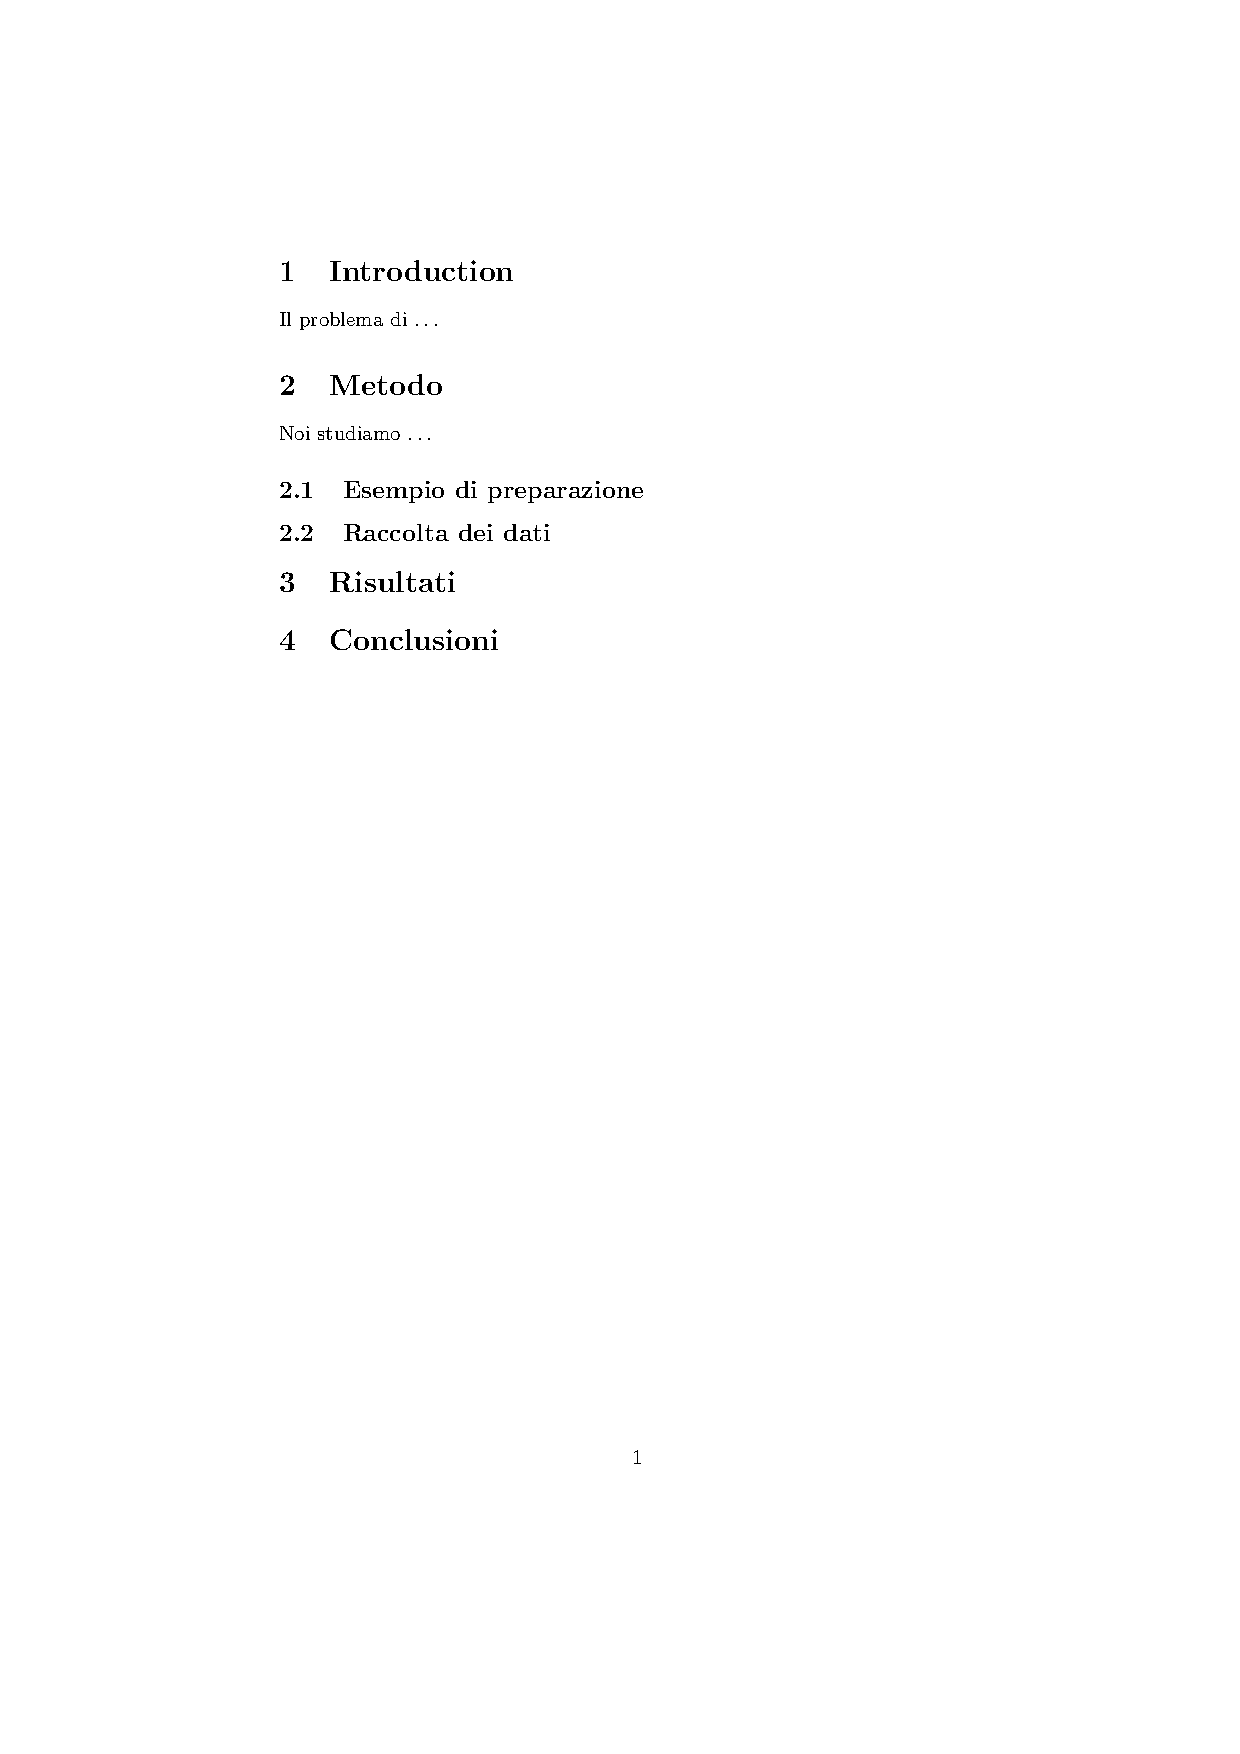
\includegraphics[width=\textwidth,clip,trim=1.5in 6in 4in 1in]{A2022.IDSEPCLaTeX/struttura-sezione.pdf}
\end{minipage}
\end{frame}

%%%%%%%%%%%%%%%%%%%%%%%%%%%%%%%%%%%%%%%%%%%%%%%%%%%%%%%%%%%%%%%%%%%%%%%%%%%%%%%
%%%%%%%%%%%%%%%%%%%%%%%%%%%%%%%%%%%%%%%%%%%%%%%%%%%%%%%%%%%%%%%%%%%%%%%%%%%%%%%
%%%%%%%%%%%%%%%%%%%%%%%%%%%%%%%%%%%%%%%%%%%%%%%%%%%%%%%%%%%%%%%%%%%%%%%%%%%%%%%
\subsection{\centerline{Etichette (\cmdbs{label}) e riferimenti incrociati}}
\begin{frame}[fragile]{\insertsubsection}
\begin{itemize}{\small
\item Si usano i comandi \cmdbs{label} e \cmdbs{ref} .
\item Nel package \bftt{amsmath} c'\`{e} \cmdbs{eqref} per far riferimento a equazioni.
}\end{itemize}
\begin{minipage}{0.55\linewidth}
\inputminted[fontsize=\scriptsize,frame=single,resetmargins]{latex}%
  {A2022.IDSEPCLaTeX/struttura-riferimenti-incrociati.tex}
\end{minipage}
\begin{minipage}{0.35\linewidth}
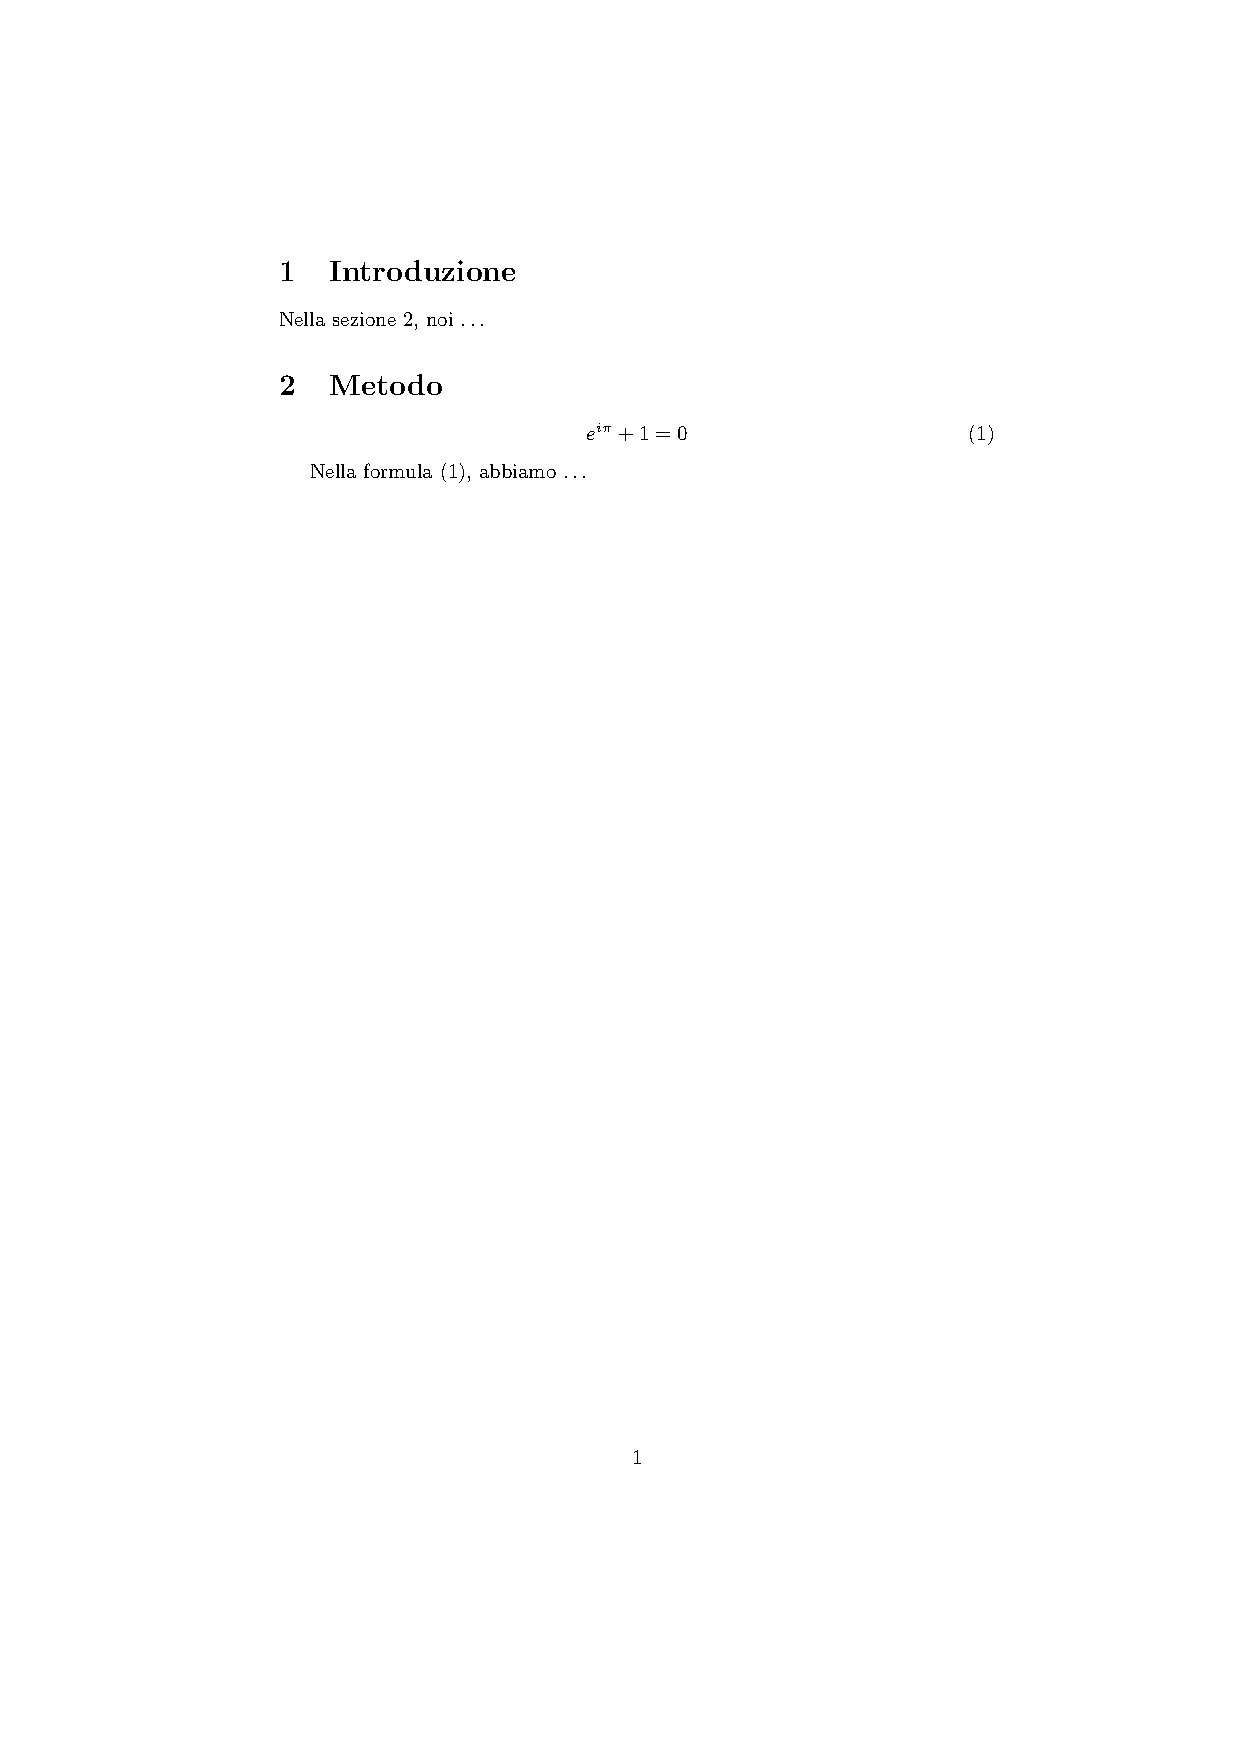
\includegraphics[width=\textwidth,clip,trim=1.8in 6in 1.6in 1in]{A2022.IDSEPCLaTeX/struttura-riferimenti-incrociati.pdf}
\end{minipage}
\end{frame}

%%%%%%%%%%%%%%%%%%%%%%%%%%%%%%%%%%%%%%%%%%%%%%%%%%%%%%%%%%%%%%%%%%%%%%%%%%%%%%%
%%%%%%%%%%%%%%%%%%%%%%%%%%%%%%%%%%%%%%%%%%%%%%%%%%%%%%%%%%%%%%%%%%%%%%%%%%%%%%%
%%%%%%%%%%%%%%%%%%%%%%%%%%%%%%%%%%%%%%%%%%%%%%%%%%%%%%%%%%%%%%%%%%%%%%%%%%%%%%%
\begin{frame}[fragile]{\centerline{Esercizi sui documenti strutturati}}
\begin{itemize}
    \item 
Scrivi questo articolo in \LaTeX:
\footnote{Da \url{http://pdos.csail.mit.edu/scigen/}, un generatore randomico di testi, tradotto ed adattato dal docente.}

\vskip 4ex
\begin{center}
\fbox{\href{\fileuri/struttura-esercizio-soluzione.pdf}{%
Cliccare qui per visualizzare l'articolo.}}
\end{center}

\vskip 4ex
Formattare l'articolo come questo modello. Usare \cmdbs{ref} e \cmdbs{eqref} per evitare di scrivere in modo esplicito i numeri di sezione e di equazione.

\vskip 4ex
\begin{center}
\fbox{\href{\wlnewdoc{struttura-esercizio.tex}}{%
Cliccare qui per aprire l'esercizio in \wllogo{}}}
\end{center}
\end{itemize}
\vskip 2ex
\begin{itemize}
\item Completato l'esercizio,
\fbox{\href{\wlnewdoc{struttura-esercizio-soluzione.tex}}{%
qui c'\`{e} una soluzione}}.
\end{itemize}
\end{frame}


\begin{frame}[fragile]{\centerline{La grafica}}
\begin{itemize}
\item È necessario caricare il pacchetto \bftt{graphicx}, in quanto fornize il comando
\cmdbs{includegraphics}.
\item I formati gestiti sono JPEG, PNG e PDF (di solito).
\end{itemize}
\vskip 4ex
\begin{exampletwouptiny}

\includegraphics[
  width=0.5\textwidth]{A2022.IDSEPCLaTeX/gerbil}


\includegraphics[
  width=0.3\textwidth,
  angle=270]{gerbil}
\end{exampletwouptiny}

\tiny{Licenza per l'immagine: \href{https://pixabay.com/en/animal-apple-attractive-beautiful-1239390/}{CC0}}
\end{frame}

%%%%%%%%%%%%%%%%%%%%%%%%%%%%%%%%%%%%%%%%%%%%%%%%%%%%%%%%%%%%%%%%%%%%%%%%%%%%%%%
%%%%%%%%%%%%%%%%%%%%%%%%%%%%%%%%%%%%%%%%%%%%%%%%%%%%%%%%%%%%%%%%%%%%%%%%%%%%%%%
%%%%%%%%%%%%%%%%%%%%%%%%%%%%%%%%%%%%%%%%%%%%%%%%%%%%%%%%%%%%%%%%%%%%%%%%%%%%%%%
\begin{frame}[fragile]{Gli argomenti opzionali}
\begin{itemize}
\item Per gli argomenti opzionali usiamo le parentesi quadre \keystrokebftt{[} \keystrokebftt{]} invece delle parentesi graffe \keystrokebftt{\{} \keystrokebftt{\}}.
\item \cmdbs{includegraphics} accetta argomenti opzionali che permettono di modificare l'immagine una volta che \`{e} stata inclusa.

Per esempio, \bftt{width=0.5\cmdbs{textwidth}} fa in modo che la larghezza dell'immagine sia il 50\% della larghezza del testo  (\cmdbs{textwidth}).
\item \cmdbs{documentclass} pure accetta argomenti opzioni:
\mint{latex}|\documentclass[12pt,twocolumn]{article}|
rende il carattere del testo pi\`{u} grande (12pt) and puts e dispone il testo su due colonne.
\item Ulteriori informazioni su dove reperire queste informazioni sono provviste nel seguito.
\end{itemize}
\end{frame}

%%%%%%%%%%%%%%%%%%%%%%%%%%%%%%%%%%%%%%%%%%%%%%%%%%%%%%%%%%%%%%%%%%%%%%%%%%%%%%%
%%%%%%%%%%%%%%%%%%%%%%%%%%%%%%%%%%%%%%%%%%%%%%%%%%%%%%%%%%%%%%%%%%%%%%%%%%%%%%%
%%%%%%%%%%%%%%%%%%%%%%%%%%%%%%%%%%%%%%%%%%%%%%%%%%%%%%%%%%%%%%%%%%%%%%%%%%%%%%%
\begin{frame}{\centerline{Flottanti}}
\begin{itemize}
\item Quando si tratta di scegliere la posizione di una figura \~{e} meglio lasciare \LaTeX{} a decidere dove la posizione, cio\~{e} lasciarla ``flottante''.
\item Si pu\`{o} aggiungere una didascalia (in inglese \bftt{caption}) alla figura, che poi pu\`{o} essere utilizzata per un riferimento con
\cmdbs{ref}.
\end{itemize}
\begin{minipage}{0.55\linewidth}
\inputminted[fontsize=\scriptsize,frame=single,resetmargins]{latex}%
  {A2022.IDSEPCLaTeX/inserimento-figura.tex}
\end{minipage}
\begin{minipage}{0.35\linewidth}
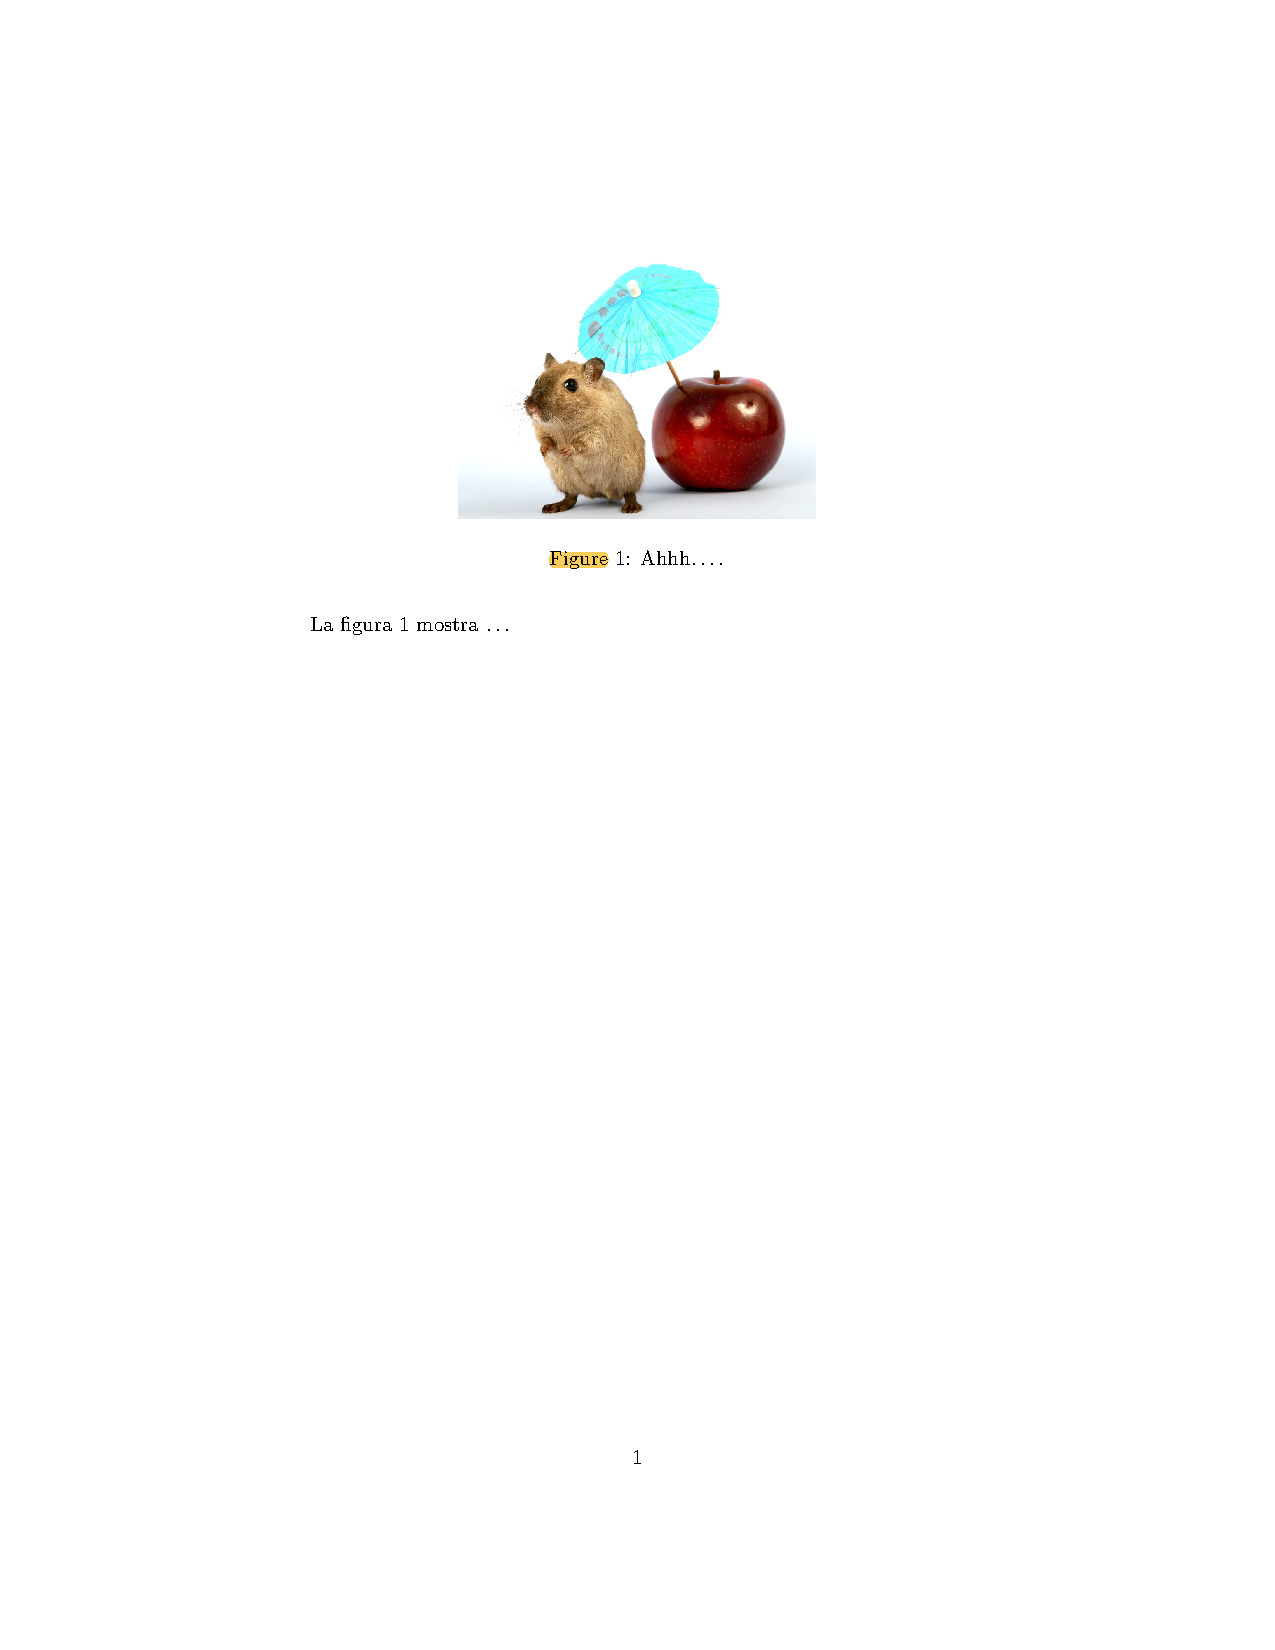
\includegraphics[width=\textwidth,clip,trim=2in 5in 3in 1in]{A2022.IDSEPCLaTeX/inserimento-figura.pdf}
\end{minipage}

\tiny{Licenza per l'immagine: \href{https://pixabay.com/en/animal-apple-attractive-beautiful-1239390/}{CC0}}
\end{frame}

%%%%%%%%%%%%%%%%%%%%%%%%%%%%%%%%%%%%%%%%%%%%%%%%%%%%%%%%%%%%%%%%%%%%%%%%%%%%%%%
%%%%%%%%%%%%%%%%%%%%%%%%%%%%%%%%%%%%%%%%%%%%%%%%%%%%%%%%%%%%%%%%%%%%%%%%%%%%%%%
%%%%%%%%%%%%%%%%%%%%%%%%%%%%%%%%%%%%%%%%%%%%%%%%%%%%%%%%%%%%%%%%%%%%%%%%%%%%%%%
\begin{frame}[fragile]{\centerline{Tabelle (1/2)}}
\begin{itemize}
\item Le tabelle \LaTeX{} non sono semplicissime; chi ha usato HTML o (t/n)roff \`{e} indubbiamente facilitato.
\item Si usa l'ambiente \bftt{tabular} che viene ulteriormente specificato nel pacchetto \bftt{tabularx}.
\item L'argomento specifica l'allineamento --- \textbf{l}eft, \textbf{c}enter, \textbf{r}ight.
\vskip 4ex
\begin{exampletwouptiny}
\begin{tabular}{lrr}
Tipo   & Numero &  \euro \\
Maniglia & 1   & 49  \\
Porta & 2   & 99  \\
Cavo  & 3   & 19   \\
\end{tabular}
\end{exampletwouptiny}
\item Si usa la ``e commerciale'' \keystrokebftt{\&} per separare le colonne e la doppia barra inversa \keystrokebftt{\bs}\keystrokebftt{\bs} per un a capo, esattamente come nell'ambiente \bftt{align*}.
\end{itemize}
\end{frame}

\begin{frame}[fragile]{\centerline{Tabelle (2/2)}}
\begin{itemize}
\item Per specificare linee orizzontali occorre usare \cmdbs{hline}.
\item Le linee verticali sono specificati con una barretta \keystrokebftt{\textbar} tra le definizioni delle colonne del \bftt{tabular}.
\vskip 4ex

\begin{exampletwouptiny}
\begin{tabular}{|l|r|r|} \hline
Elemento   & Quantit\`{a} & \euro \\\hline
Widget & 1   & 49  \\
Gadget & 2   & 99  \\
Cable  & 3   & 19   \\\hline
\end{tabular}
\end{exampletwouptiny}
\item Si noti che
\begin{itemize}
\item il simbolo di euro pu\`{o} essere realizzato con il comando \cmdbs{euro} e l'uso del pacchetto  \bftt{eurosym}.
\item la barretta verticale pu\`{o} essere realizzata con il comando \cmdbs{textbar}.
\end{itemize}
\end{itemize}
\end{frame}



%%%%%%%%%%%%%%%%%%%%%%%%%%%%%%%%%%%%%%%%%%%%%%%%%%%%%%%%%%%%%%%%%%%%%%%%%%%%%%%
%%%%%%%%%%%%%%%%%%%%%%%%%%%%%%%%%%%%%%%%%%%%%%%%%%%%%%%%%%%%%%%%%%%%%%%%%%%%%%%
%%%%%%%%%%%%%%%%%%%%%%%%%%%%%%%%%%%%%%%%%%%%%%%%%%%%%%%%%%%%%%%%%%%%%%%%%%%%%%%
\begin{frame}[fragile]{\centerline{bib\TeX (1/3)}}
\begin{itemize}
\item I riferimenti bibliografici possono essere gestiti in modo efficace con il sistema bib\TeX.
\item Occorre mettere i riferimenti in un file \bftt{.bib} in formato `bibtex':
\inputminted[fontsize=\scriptsize,frame=single]{latex}{A2022.IDSEPCLaTeX/bib-esempio.bib}
\end{itemize}
\end{frame}

%%%%%%%%%%%%%%%%%%%%%%%%%%%%%%%%%%%%%%%%%%%%%%%%%%%%%%%%%%%%%%%%%%%%%%%%%%%%%%%
%%%%%%%%%%%%%%%%%%%%%%%%%%%%%%%%%%%%%%%%%%%%%%%%%%%%%%%%%%%%%%%%%%%%%%%%%%%%%%%
%%%%%%%%%%%%%%%%%%%%%%%%%%%%%%%%%%%%%%%%%%%%%%%%%%%%%%%%%%%%%%%%%%%%%%%%%%%%%%%
\begin{frame}[fragile]{\centerline{bib\TeX (2/3)}}
\begin{itemize}
\item La maggior parte dei sistemi di gestione delle bibliografie possono esportare in formato bibtex.
\item Ogni elemento nel file \bftt{.bib} ha una \emph{chiave} per far riferimento ad esso nel testo. Per esempio, \bftt{Jacobson1999Towards} \`{e} la chiave per l'articolo:
\begin{minted}[fontsize=\small,frame=single]{latex}
@Article{Jacobson1999Towards,
  author = {Van Jacobson},
  ...
}
\end{minted}
\item \`{E} una buona idea usare una chiave legata a nome, titolo e anno.
\item \LaTeX{} formatta automaticamente la citazione e genera la bibliografia; conosce la maggior parte degli standard bibliografici e comunque pu\`{o} essere customizzato.
\end{itemize}
\end{frame}

%%%%%%%%%%%%%%%%%%%%%%%%%%%%%%%%%%%%%%%%%%%%%%%%%%%%%%%%%%%%%%%%%%%%%%%%%%%%%%%
%%%%%%%%%%%%%%%%%%%%%%%%%%%%%%%%%%%%%%%%%%%%%%%%%%%%%%%%%%%%%%%%%%%%%%%%%%%%%%%
%%%%%%%%%%%%%%%%%%%%%%%%%%%%%%%%%%%%%%%%%%%%%%%%%%%%%%%%%%%%%%%%%%%%%%%%%%%%%%%
\begin{frame}[fragile]{\centerline{bib\TeX (3/3)}}
\begin{itemize}
\item \`{E} conveniente usare il pacchetto \bftt{natbib} \footnote{C'\`{e} un nuovo pacchetto con funzionalit\`{a} aggiuntive chiamato \bftt{biblatex} ma la maggior parte degli articoli usano ancora
  \bftt{natbib}.} con \cmdbs{citet} e \cmdbs{citep}.
\item Utilizzare \cmdbs{bibliography} alla fine e specificare un \cmdbs{bibliographystyle}.
\end{itemize}
\begin{minipage}{0.55\linewidth}
\inputminted[fontsize=\scriptsize,frame=single,resetmargins]{latex}%
  {A2022.IDSEPCLaTeX/bib-esempio.tex}
\end{minipage}
\begin{minipage}{0.35\linewidth}
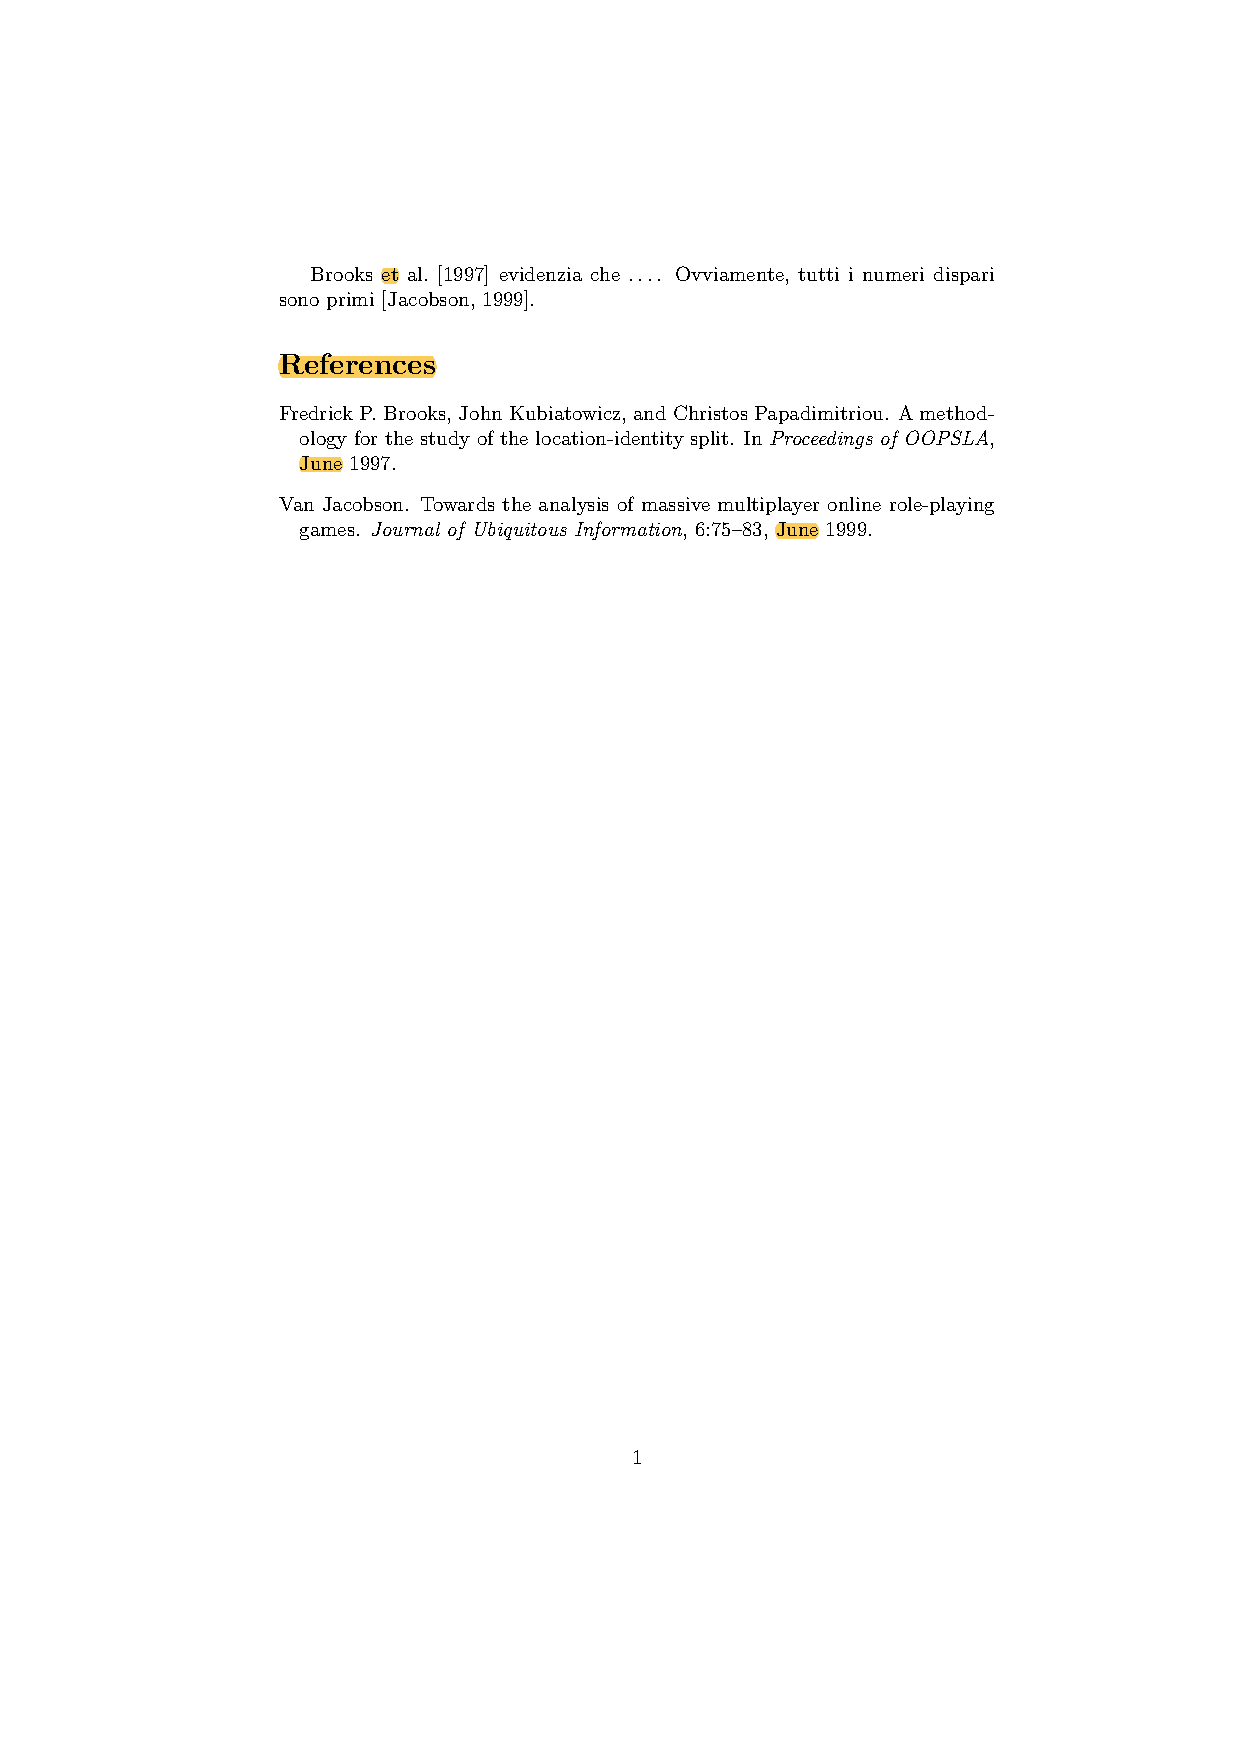
\includegraphics[width=\textwidth,clip,trim=1.8in 5in 1.8in 1in]{A2022.IDSEPCLaTeX/bib-esempio.pdf}
\end{minipage}
\end{frame}

\begin{frame}[fragile]{\centerline{Esercizio riassuntivo}}

Aggiungere una immagine e la bibliografia all'esercizio precedente.


\begin{enumerate}
\item Scaricare questi file di esempio sul proprio computer.
\vskip 4ex

\begin{center}
\fbox{\href{\fileuri/gerbil.jpg?dl=1}{Cliccare per scaricare l'immagine di esempio}}
\vskip 4ex

\fbox{\href{\fileuri/bib-esercizio.bib?dl=1}{Cliccare per scaricare il file bib di esempio}}
\end{center}
\vskip 4ex

\item Caricare i file su \wllogo.

\end{enumerate}
\end{frame}


%%%%%%%%%%%%%%%%%%%%%%%%%%%%%%%%%%%%%%%%%%%%%%%%%%%%%%%%%%%%%%%%%%%%%%%%%%%%%%%
%%%%%%%%%%%%%%%%%%%%%%%%%%%%%%%%%%%%%%%%%%%%%%%%%%%%%%%%%%%%%%%%%%%%%%%%%%%%%%%
%%%%%%%%%%%%%%%%%%%%%%%%%%%%%%%%%%%%%%%%%%%%%%%%%%%%%%%%%%%%%%%%%%%%%%%%%%%%%%%
\subsection{\centerline{Alcuni comandi interessanti}}
\begin{frame}[fragile]{\insertsubsection}
\begin{itemize}
\item Con \cmdbs{tableofcontents} si genera un indice (in inglese ``Table of Content''
dai comandi di sezione \cmdbs{section}.

\item Si pu\`{o} radicalmente cambiare la formattazione cambiando argomento di \cmdbs{documentclass} ad esempio in
\mint{latex}!\documentclass{scrartcl}!
o in
\mint{latex}!\documentclass[12pt]{IEEEtran}!

\item Si possono definire i propri comandi per formule complesse, semplificando la scrittura:
\begin{exampletwouptiny}
\newcommand{\rperf}{%
  \rho_{\text{perf}}}
$$
\rperf = {\bf c}'{\bf X} + \varepsilon
$$
\end{exampletwouptiny}
\end{itemize}
\end{frame}

%%%%%%%%%%%%%%%%%%%%%%%%%%%%%%%%%%%%%%%%%%%%%%%%%%%%%%%%%%%%%%%%%%%%%%%%%%%%%%%
%%%%%%%%%%%%%%%%%%%%%%%%%%%%%%%%%%%%%%%%%%%%%%%%%%%%%%%%%%%%%%%%%%%%%%%%%%%%%%%
%%%%%%%%%%%%%%%%%%%%%%%%%%%%%%%%%%%%%%%%%%%%%%%%%%%%%%%%%%%%%%%%%%%%%%%%%%%%%%%
\begin{frame}{\centerline{Alcuni pacchetti utili}}
\begin{itemize}
\item \bftt{beamer}: presentazioni (come questa!)
\item \bftt{todonotes}: gestione di commenti e TODO
\item \bftt{tikz}: grafica
\item \bftt{pgfplots}: creare grafici
\item \bftt{listings}: codice
\item \bftt{spreadtab}: fogli elettronici
\item \bftt{gchords}, \bftt{guitar}: chitarra
\item \bftt{cwpuzzle}: parole incrociate
\end{itemize}
Si trovano esempi di questi pacchetti ai siti \url{https://www.overleaf.com/latex/examples} e \url{http://texample.net}.
\end{frame}

%%%%%%%%%%%%%%%%%%%%%%%%%%%%%%%%%%%%%%%%%%%%%%%%%%%%%%%%%%%%%%%%%%%%%%%%%%%%%%%
\begin{frame}{\centerline{Installazione \LaTeX{}}}
\begin{itemize}
\item Si pu\`{o} usare \LaTeX{} online su \wllogo, ma \ldots se non si \`{e} online?
\item Se volete avere \LaTeX{} sempre a disposizione sul vostro computer occorre scaricare una 
\emph{distribuzione}. Una distribuzione include il programma \bftt{latex} e, di solito, qualche migliaia di pacchetti.
\begin{itemize}
\item Per Windows: \href{http://miktex.org/}{Mik\TeX} o \href{http://tug.org/texlive/}{\TeX Live}
\item Per Linux: \href{http://tug.org/texlive/}{\TeX Live}
\item Per MacOS: \href{http://tug.org/mactex/}{Mac\TeX}
\end{itemize}
\item C'\`{e} anche bisogno di un editor di testi con supporto per \LaTeX{}. Un confronto tra possibili opzioni si trova alla pagina: \url{http://en.wikipedia.org/wiki/Comparison_of_TeX_editors}.
\end{itemize}
\end{frame}

%%%%%%%%%%%%%%%%%%%%%%%%%%%%%%%%%%%%%%%%%%%%%%%%%%%%%%%%%%%%%%%%%%%%%%%%%%%%%%%
%%%%%%%%%%%%%%%%%%%%%%%%%%%%%%%%%%%%%%%%%%%%%%%%%%%%%%%%%%%%%%%%%%%%%%%%%%%%%%%
%%%%%%%%%%%%%%%%%%%%%%%%%%%%%%%%%%%%%%%%%%%%%%%%%%%%%%%%%%%%%%%%%%%%%%%%%%%%%%%
\begin{frame}{\centerline{Risorse disponibili online}}
\begin{itemize}
\item \href{https://www.overleaf.com/learn}{Il Wiki per imparare Overleaf} ---
Presentazioni, tutorial, e manuali aggiuntivi
\item \href{http://en.wikibooks.org/wiki/LaTeX}{The \LaTeX{} Wikibook} ---
Una collezione di tutorial e materiale di riferimento.
\item \href{http://tex.stackexchange.com/}{\TeX{} Stack Exchange} --- Domande e risposte tipiche, ma anche la possibilit\`{a} di fare domande ed avere risposte in tempi brevi, se si \`{e} fortunati
\item \href{http://www.latex-community.org/}{\LaTeX{} Community} --- un grande forum online
\item \href{http://ctan.org/}{Comprehensive \TeX{} Archive Network (CTAN)} --- La complete rete di archivi di \TeX{}. pi\`{u} di quattromila pacchetti e documentazoini
\item Google !
\end{itemize}
\end{frame}

%%%%%%%%%%%%%%%%%%%%%%%%%%%%%%%%%%%%%%%%%%%%%%%%%%%%%%%%%%%%%%%%%%%%%%%%%%%%%%%

\begin{frame}[fragile]{\centerline{Esercizio conclusivo}}

\begin{enumerate}
\item Qui c'\`{e} un breve testo copiato, tradotto e rielaborato da  \url{http://www.cgd.ucar.edu/cms/agu/scientific_talk.html}
\vskip 2ex
\begin{center}
\fbox{\href{\wlnewdoc{struttura-esercizio.tex}}{%
Cliccare qui per aprire il documento in \wllogo{}}}
\end{center}
\vskip 2ex
\item Aggiungi i comandi \LaTeX{} per rendere il testo pi\`{u} simile possibile a questo:
\begin{center}
\fbox{\href{\fileuri/recap-exercise-solution.pdf}, ricordarsi di premettere la barretta inversa (\cmdbs{\%}).
\item Nelle formule, usare \cmdbs{frac} per le frazioni.
\end{itemize}
\end{enumerate}

\end{frame}


\end{document}

